\documentclass[t,xcolor={usenames,dvipsnames}]{beamer}

\mode<presentation>
{
\usetheme{Frankfurt}%{Warsaw}
%\setbeamercovered{transparent}
%\setbeamercolor{background canvas}{bg=white}
}

% Delete these, if you do not want the table of contents to pop up at
% the beginning of each (sub)section:
%\AtBeginSubsection[]
%{
%  \begin{frame}<beamer>{Outline}
%    \tableofcontents[currentsection,currentsubsection]
%  \end{frame}
%}
%\AtBeginSection[]
%{
%  \begin{frame}<beamer>{Outline}
%    \tableofcontents[currentsection]
%  \end{frame}
%}

\usepackage[english]{babel}
\usepackage[latin1]{inputenc}
\usepackage{times}
\usepackage[T1]{fontenc}
\usepackage{verbatim}
\usepackage{url}
\usepackage{amsmath,amssymb}
\usepackage{comment}
\usepackage[overlay,absolute]{textpos}
\usepackage{hyperref}

% Author-date citations
\usepackage[authoryear,round]{natbib}
\let\cite=\citep  % default \cite such as {\LaTeX} authors are used to

% Where \includegraphics should look for figures
\graphicspath{{./figs/}}
\usepackage{epstopdf}
\DeclareGraphicsExtensions{.eps,.png,.jpg,.pdf}

% Shortcuts
\newcommand{\myhref}[2]{\href{#1}{\textcolor{Blue}{#2}}}
\newcommand{\myurl}[1]{\myhref{#1}{#1}}
\newcommand{\subitem}[1]{\begin{itemize}[<.->]\item #1 \end{itemize}}
\newcommand{\ghead}[1]{{\tiny #1\\}}
\newcommand{\doi}[1]{\myhref{http://dx.doi.org/#1}{doi:#1}}
\newcommand{\csym}[1]{\textcolor{Blue}{\texttt{#1}}}
\newcommand{\ud}{\mathrm{d}}
\newcommand{\dt}{\ud t}

%%%%%%%%%%%%%%%%%%%%%%%%%%%%%%%%%%%%%%%%%%%%%%%%%%%%%%%%%%%%%%%%%%%%%%
\title{Functional Curation of Mathematical Models}
\author{Jonathan Cooper}
\institute[University of Oxford]
{Computational Biology Group\\
 Department of Computer Science\\
 University of Oxford}
\date{February 8, 2013}

\begin{document}

\begin{frame}
\titlepage
\end{frame}

\begin{comment}
This is a 10 minute intro for the 2020 Tools Workshop.
It will be followed by a demo over lunch.
The main Chaste intros and demos are after lunch.
\end{comment}

%%%%%%%%%%%%%%%%%%%%%%%%%%%%%%%%%%%%%%%%%%%%%%%%%%%%%%%%%%%%%%%%%%%%%%

%\begin{frame}{Outline}
%\setcounter{tocdepth}{1}
%\tableofcontents
%\end{frame}

%%%%%%%%%%%%%%%%%%%%%%%%%%%%%%%%%%%%%%%%%%%%%%%%%%%%%%%%%%%%%%%%%%%%%%
\section{Introduction to functional curation}
\subsection*{Main}
%%%%%%%%%%%%%%%%%%%%%%%%%%%%%%%%%%%%%%%%%%%%%%%%%%%%%%%%%%%%%%%%%%%%%%

\begin{frame}{Setting the context}
\begin{itemize}
\item Model reuse \& simulation result reproducibility
\item Improving the modelling process
\item Confronting models with data
\end{itemize}
\end{frame}


\begin{frame}{Setting the context}
\begin{itemize}
\item Many models are available in languages such as CellML
\item But, how can we\ldots
  \begin{itemize}
  \item Determine a model's functionality, i.e.\ its suitability or limitations for a new study?
  \item Re-use a model in a different experimental context?
  \item Compare different models' behaviours under the same experiment?  (Compare hypotheses.)
  \end{itemize}
\end{itemize}
\end{frame}


\begin{frame}{Goal of this work}
\begin{itemize}
\item Provide a framework for a coherent approach to model fitting, simulation, comparison and validation
  \begin{itemize}
  \item Continuous evaluation of model predictions against experimental data, throughout model lifecycle
  \item Models that are robust, well tested, and well characterised for particular biological studies
  \item Model development akin to high quality software
  \end{itemize}
\end{itemize}
\end{frame}


\begin{frame}{How do we get there?}
\subitem{Separate \alert{model structure} and \alert{experimental scenario}}
\begin{center}
\includegraphics[width=.9\textwidth]{VirtEx_overview}
\end{center}
\subitem{Tooling to run protocols on models, generate graphs, etc.}
\end{frame}


\begin{frame}{What goes in a protocol?}
\begin{center}
\includegraphics[width=\textwidth]{protocol_language}
\end{center}
\end{frame}


%%%%%%%%%%%%%%%%%%%%%%%%%%%%%%%%%%%%%%%%%%%%%%%%%%%%%%%%%%%%%%%%%%%%%%
\section{Examples}
\subsection*{Main}
%%%%%%%%%%%%%%%%%%%%%%%%%%%%%%%%%%%%%%%%%%%%%%%%%%%%%%%%%%%%%%%%%%%%%%

\begin{frame}{Cardiac example: S1-S2 restitution}
\begin{center}
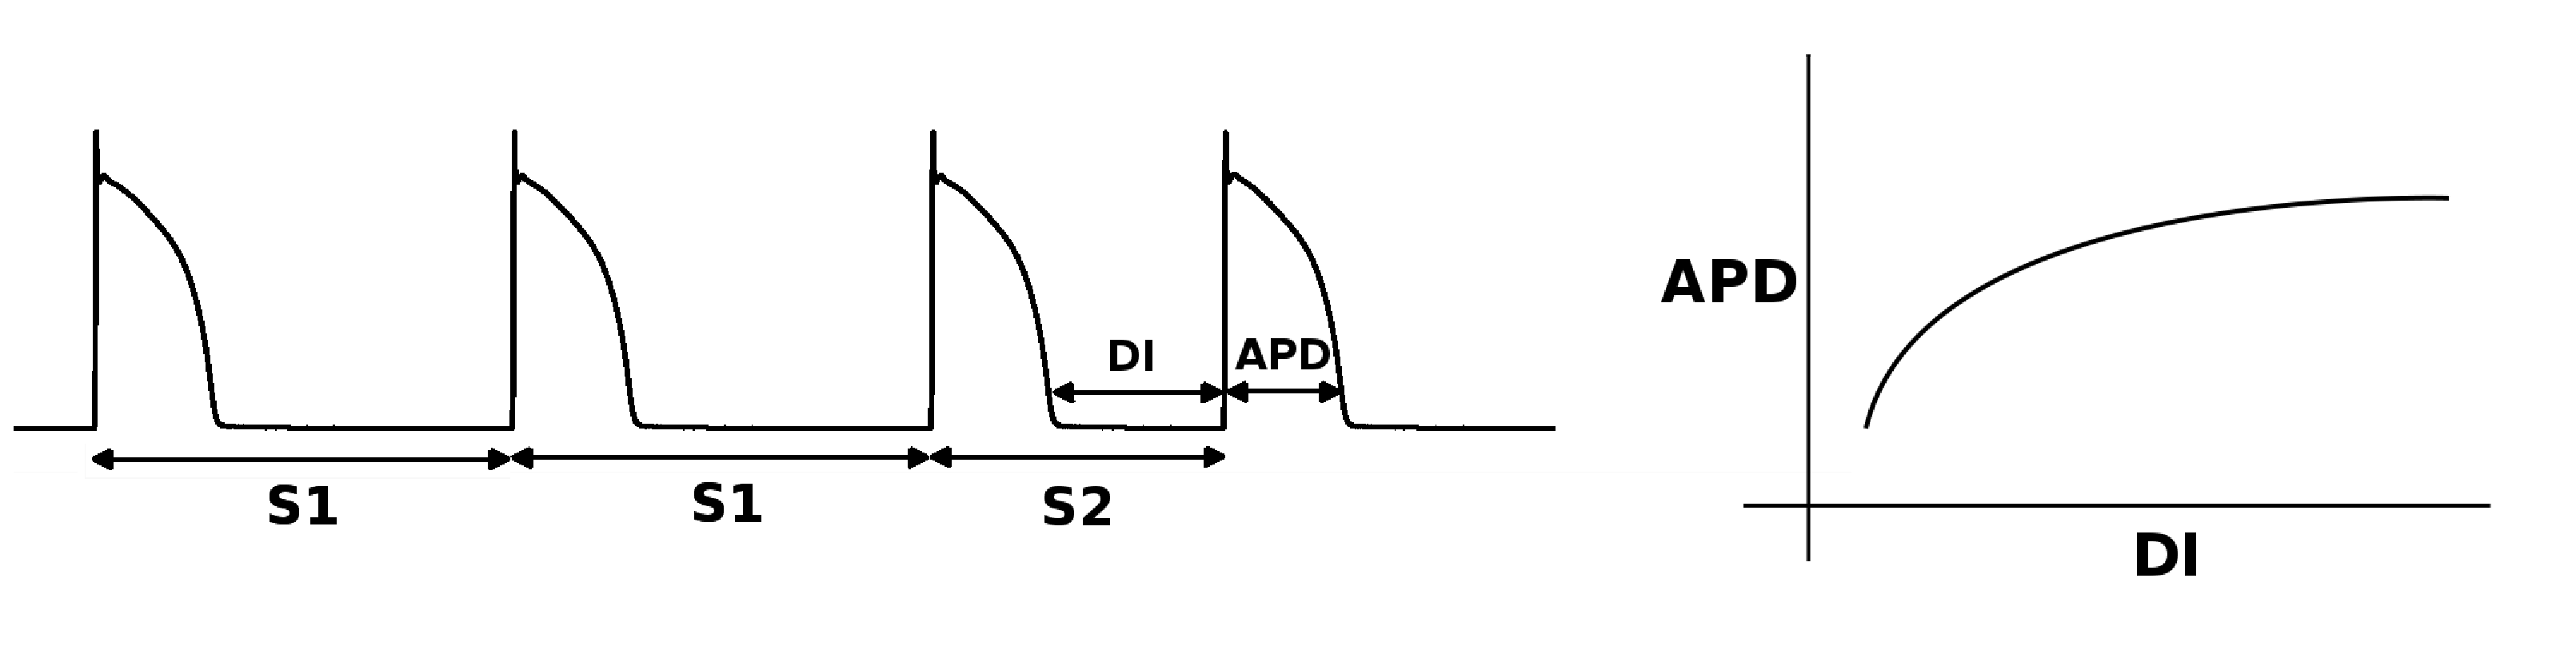
\includegraphics[width=\textwidth]{S1S2}
\end{center}
\end{frame}


\begin{frame}{S1-S2 restitution on canine models}
\begin{columns}[T]
\begin{column}{.33\linewidth}
\begin{center}
\includegraphics[width=\textwidth]{sicouri_dog_ventricle_s1s2_curve}\\
\vspace{.1cm}
\includegraphics[width=\textwidth]{hund_rudy_2004_s1s2_curve}
\end{center}
\end{column}
\begin{column}{.33\linewidth}
\begin{center}
\includegraphics[width=\textwidth]{winslow_model_1999_s1s2_curve}\\
\vspace{.1cm}
\includegraphics[width=\textwidth]{livshitz_rudy_2007_s1s2_curve}
\end{center}
\end{column}
\begin{column}{.33\linewidth}
\begin{center}
\includegraphics[width=\textwidth]{fox_mcharg_gilmour_2002_s1s2_curve}\\
\vspace{.1cm}
\includegraphics[width=\textwidth]{decker_2009_s1s2_curve}
\end{center}
\end{column}
\end{columns}
\end{frame}


\begin{frame}{Case study linking to cell-based Chaste}
\centering
\begin{minipage}{0.28\textwidth}
\includegraphics[width=.9\textwidth]{VariableWnt}
\end{minipage}
\begin{minipage}{0.39\textwidth}
\includegraphics[width=.9\textwidth]{WongFigure}
\end{minipage}
\begin{minipage}{0.31\textwidth}
\begin{itemize}
\item Cell division locations in intestinal crypt
\item Compare three submodels for cell cycle
\item Parameter sweep over crypt height
\end{itemize}
\end{minipage}
\end{frame}


\begin{frame}{Results}
\vspace{-.45cm}
{\footnotesize Distributions of crypt cell division events with different cell cycle models}
\vspace{-.1cm}
\hspace*{2mm}
\includegraphics[width=.45\textwidth]{Uniform_Wnt-Cell_division_locations}
\hspace*{5mm}
\includegraphics[width=.45\textwidth]{Variable_Wnt-Cell_division_locations}\\
\hspace*{2mm}
\includegraphics[width=.45\textwidth]{Stochastic_Generation-based-Cell_division_locations}
\hspace*{12mm}
\includegraphics[height=.4\textheight]{WongFigure}
\end{frame}


%%%%%%%%%%%%%%%%%%%%%%%%%%%%%%%%%%%%%%%%%%%%%%%%%%%%%%%%%%%%%%%%%%%%%%
\begin{frame}{Acknowledgments}
Gary Mirams, James Osborne\\
Chaste team\\
Alan Garny, Steven Niederer, David Gavaghan

Reference publication: \doi{10.1016/j.pbiomolbio.2011.06.003}\\
Website: \myurl{https://chaste.cs.ox.ac.uk/trac/wiki/FunctionalCuration}

\begin{center}
\includegraphics[scale=.9]{chaste-266x60}\\ \vspace{.3cm}
\includegraphics[scale=.7]{logo2020science}\\ \vspace{.4cm}
\includegraphics[width=.55\textwidth]{EPSRC1RGBLO} \hspace{.1cm}
\includegraphics[scale=.55]{logo_msr}
\end{center}
\end{frame}


\end{document}
